% ==========================================================
\chapter{Background}
\label{chapter:background}
% ==========================================================

This chapter establishes the theoretical foundations of this thesis.
It introduces behavioral programming and feature modeling as the core conceptual pillars.
Building on this, it explains \textit{models@run.time} as the perspective on runtime adaptation and presents the Graphical Language Server Platform as the technological basis for graphical model tooling.
It concludes with the visual representation theory, which grounds the design rationale for cognitively effective diagram notations.

\glsresetall

% ==========================================================
\section{Behavioral Programming}
\label{sec:bp}
% ==========================================================

\gls{bp} is a paradigm for programming reactive systems~\cite{harel_behavioral_2012}.
It bridges the gap between requirements and implementation by expressing system behavior as executable scenarios and use cases.
\gls{bp} is based on independent scenarios that correspond to individual system requirements.
Given that each scenario acts as a standalone module, developers can incrementally extend and refine the system by adding new behaviors, rules, or tactics without changing existing code.
This development style makes \gls{bp} well-suited for complex, reactive systems~\cite{elyasaf_context-oriented_2021}.

% ----------------------------------------------------------
\subsection{Foundations of Behavioral Programming}
\label{subsec:bp_foundation}
% ----------------------------------------------------------

The primary building blocks of \gls{bp} are behavioral threads (b-threads)~\cite{harel_behavioral_2012}.
Each b-thread runs concurrently and captures one specific scenario that the system should or should not follow.
The b-threads are decoupled and typically do not know of one another.

B-threads communicate through an enhanced publish/subscribe protocol using the \texttt{bSync} method~\cite{harel_behavioral_2012}.
When a b-thread reaches a synchronization point, it invokes \texttt{bSync} and suspends execution until the arbiter evaluates the joint state of all b-threads.
At each synchronization point, every b-thread submits three sets of events to the event arbiter:
\begin{itemize}
\item \textbf{requested:} The b-thread proposes these events for execution and asks to be notified if they occur.
\item \textbf{waited-for:} These events are not triggered by the b-thread, but it asks to be notified if another thread successfully requests them.
\item \textbf{blocked:} The b-thread explicitly forbids these events from occurring, acting as a veto against other b-threads' requests.
\end{itemize}
An event is triggered only if at least one b-thread requests it and none block it~\cite{elyasaf_context-oriented_2021}.

% ----------------------------------------------------------
\subsection{Context-Oriented Behavioral Programming}
\label{subsec:bp_context-oriented}
% ----------------------------------------------------------

\gls{cobp}, formalized by Elyasaf~\cite{elyasaf_context-oriented_2021}, extends \gls{bp} by integrating dynamic environmental data and system state into the behavioral model.
In Harel's original \gls{bp}, systems are built from independent b-threads that communicate only by requesting, waiting for, and blocking events at synchronization points~\cite{harel_behavioral_2012}.
While this keeps threads isolated, it leaves no explicit, first-class mechanism for representing or changing context. 
As a result, sharing contextual data among b-threads requires structural workarounds~\cite{elyasaf_context-oriented_2021}.

Elyasaf addresses this in \gls{cobp} by introducing formal extensions to manage context natively.
Instead of standard b-threads, \gls{cobp} uses Context-Aware Behavioral Threads (CBTs), each bound to a query over the system's contextual data~\cite{elyasaf_context-oriented_2021}.
When a CBT's query yields a new result, the system spawns a live copy of that CBT, passing the query result as a local variable called the seed, allowing the thread to execute its logic in that specific context.
\gls{cobp} also connects behavioral events to data updates through an effect function, which translates selected events into updates to the contextual data structure before propagating the updated context to all live copies.

An empirical study suggests that this explicit context modeling helps developers comprehend complex, context-dependent guard rules~\cite{ashrov_study_2025}.
It is also well-suited for scalable systems that must adapt to changing conditions, such as smart devices and robotic controllers.
At the same time, \gls{cobp} introduces a steeper learning curve and higher cognitive load, which can make systems more difficult to comprehend and align with requirements than classical \gls{bp} does.

% ----------------------------------------------------------
\subsection{Water Tank Example}
\label{subsec:bp_water-tank}
% ----------------------------------------------------------

To illustrate \gls{bp} in a dynamic environment, Harel introduces the Water Tank scenario~\cite{harel_behavioral_2012, elyasaf_context-oriented_2021}.
The system maintains target water levels and temperatures by controlling a hot water tap, a cold water tap, and a drain.
Instead of a monolithic control structure, independent concurrent b-threads are used, each managing a single requirement.
Figure~\ref{fig:bp-water-tank} illustrates one representative runtime situation of this example.

\begin{itemize}
\item \textbf{AddHot}: Requests the \textit{HOT} event (adds hot water).
\item \textbf{AddCold}: Requests the \textit{COLD} event (adds cold water).
\item \textbf{RemoveWater}: Requests the \textit{DRAIN} event (decreases water level).
\item \textbf{ControlTank}: Acts as a supervisor that enforces operational limits by blocking specific events.
\end{itemize}

\begin{figure}
	\centering
	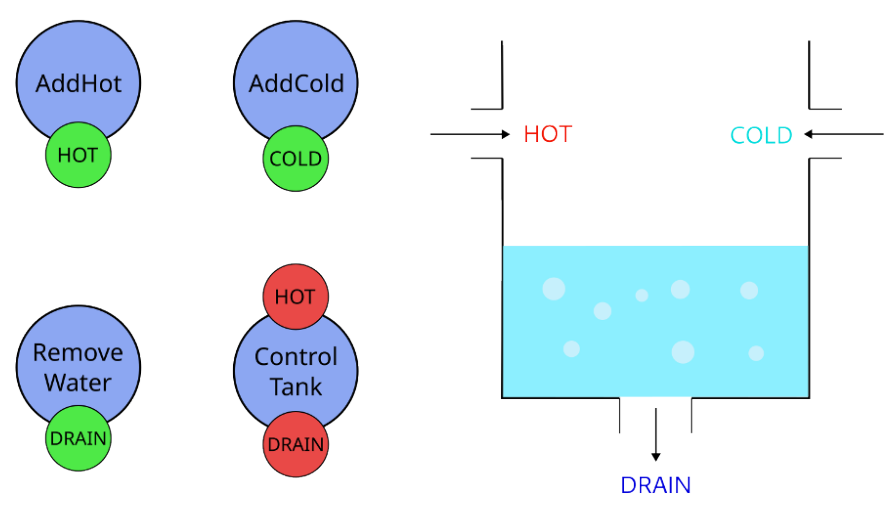
\includegraphics[width=\textwidth]{figures/bp-water-tank.png}
	\caption[Water Tank Example]{Water Tank Example; Water is too hot and too little, so \textit{HOT} and \textit{DRAIN} are blocked. Taken from \cite{felber_comprehensible_2025}.}
    \label{fig:bp-water-tank}
\end{figure}

During execution, the b-threads synchronize and vote on the next action.
An event is triggered only if it is requested and not vetoed by a supervising b-thread.
As shown in Figure~\ref{fig:bp-water-tank}, \textit{HOT} and \textit{DRAIN} are blocked in this depicted state because the water is too hot and the water level is too low.
This decoupled architecture allows developers to add new rules, such as a b-thread that prevents overflow, without altering the existing b-threads~\cite{harel_behavioral_2012}.

% ==========================================================
\section{Feature Modeling}
\label{sec:feature-modeling}
% ==========================================================

Feature modeling provides a structured way to describe commonalities and variabilities within a family of related systems.
It is central to this thesis because the proposed graphical extensions build on feature models to represent both static product structure and runtime-relevant variation.
The following subsections introduce the background of Software Product Lines, explain how feature trees encode relationships between features, and outline how \gls{uvl} captures these ideas in a textual syntax.

% ----------------------------------------------------------
\subsection{Software Product Lines}
\label{subsec:spl}
% ----------------------------------------------------------

\gls{spl} shift development from isolated systems to a reuse-oriented engineering approach~\cite{clements_software_2002}.
The core idea is to build a shared asset base that can be systematically reconfigured into a family of related products tailored to specific market needs~\cite{lee_concepts_2002}.
By managing commonality and variability across the portfolio, organizations can reduce development costs and shorten time-to-market~\cite{pohl_software_2005}.
The process is typically divided into domain engineering and application engineering~\cite{buhne_modelling_2005, apel_overview_2009}.
During domain engineering, the focus lies on defining the relevant features and constraints that characterize the product family.
Application engineering then uses this model to derive specific products tailored to individual stakeholder requirements.

\gls{dspl} extend these traditional \gls{spl} concepts by integrating both static variability in space and dynamic variability over time into a unified framework~\cite{burdek_staged_2014}.
Rather than completely shifting variability resolution away from design time, \glspl{dspl} support multiple binding times to handle features across different operational modes~\cite{capilla_overview_2014}.
This approach allows developers to clearly distinguish between static features that are finalized prior to product derivation and dynamic features that remain open as variation points.
These enable autonomous system adaptation and reconfiguration at runtime.
To manage this increased complexity and temporal dependency, developers use extended feature models that assign binding times to specific features.

Feature models in general define the boundaries of what can be built and provide a structured view of product variation, making them a natural tool for managing this variability.

% ----------------------------------------------------------
\subsection{Feature Trees}
\label{subsec:feature-trees}
% ----------------------------------------------------------

\gls{foda} established the foundation for hierarchical decomposition by defining features as user-visible characteristics identified through rigorous domain analysis~\cite{kang_feature-oriented_1990}.
A feature model consists of a hierarchically arranged collection of features.
Its structural integrity relies on the relationships between parent and child features~\cite{kang_feature-oriented_1990, czarnecki_formalizing_2005}.

Across the literature~\cite{lee_concepts_2002, czarnecki_formalizing_2005, czarnecki_staged_2004, benavides_automated_2005, benavides_automated_2010}, basic feature models contain the following relationship types:

\begin{itemize}
    \item \textbf{Mandatory.}
    A child feature has a \textit{mandatory} relationship with its parent feature if the child is part of all products in which the parent is included.
    \item \textbf{Optional.}
    A child feature has an \textit{optional} relationship with its parent feature if the child is optionally part of all products in which the parent is included.
    \item \textbf{Or.}
    A set of child features has an \textit{or} relationship with their parent feature when at least one child is active in products where the parent is included.
    \item \textbf{Alternative.}
    A set of child features has an \textit{alternative} relationship with their parent feature when exactly one child is active in products where the parent is included.
    In other literature~\cite{lee_concepts_2002, benavides_automated_2005}, the \textit{alternative} relation can be combined with \textit{mandatory} or \textit{optional}, which allows for a selection of zero elements as well.
\end{itemize}

\begin{figure}
	\centering
	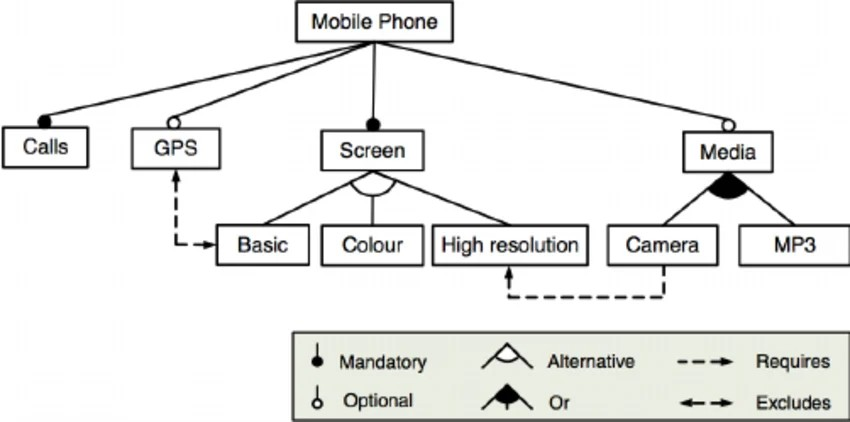
\includegraphics[width=\textwidth]{figures/feature-model.jpg}
	\caption[Example of Feature Model]{Example of a feature tree for a mobile phone, including cross-tree constraints. Taken from \cite{benavides_automated_2010}.}
    \label{fig:mobile_phone_feature_tree}
\end{figure}

Beyond these parent-child relationships, feature models may contain cross-tree constraints between features.
Typical examples are \textit{requires} and \textit{excludes}~\cite{galindo_automated_2019}.
A \textit{requires} constraint enforces that selecting one feature also requires selecting another.
An \textit{excludes} constraint stipulates that two features cannot be included in the same configuration.
More expressive formulations are also possible, including propositional constraints such as \texttt{A implies not B or not C}.
Figure~\ref{fig:mobile_phone_feature_tree} illustrates a feature tree with such cross-tree constraints.

% ----------------------------------------------------------
\subsection{Advancements to Feature Trees}
\label{subsec:advancements-to-feature-trees}
% ----------------------------------------------------------

Advanced feature modeling extends the traditional binary logic of \gls{foda} by introducing quantitative constraints and metadata.
These extensions support more complex configurations and more detailed resource tracking.

% ----------------------------------------------------------
\subsubsection{Cardinality-Based Modeling}
\label{subsubsec:cardinality-based-modeling}
% ----------------------------------------------------------

This approach borrows from \gls{uml} multiplicities to define how often and how many instances of a feature may appear in a configuration.

\textbf{Feature cardinality.}
A feature cardinality is assigned an interval $[n \dots m]$, where $n$ is the minimum and $m$ is the maximum number of instances permitted.
This generalizes traditional relationships:
\begin{itemize}
    \item Mandatory: $[1 \dots 1]$
    \item Optional: $[0 \dots 1]$
    \item Clones: Any range where $m > 1$, allowing multiple distinct instances of the same feature.
\end{itemize}

\textbf{Group cardinality.}
This restricts the selection of child features when a parent is active.
Represented by the interval $[n \dots n]$, it dictates that at least $n$ and at most $m$ children must be chosen.
This generalizes traditional relationships:
\begin{itemize}
    \item Alternative: $[1 \dots 1]$
    \item Or-Relationship: $[1 \dots k]$, where $k$ is the total number of available sub-features.
\end{itemize}

% ----------------------------------------------------------
\subsubsection{Attribute-Based Modeling}
\label{subsubsec:attribute-based-modeling}
% ----------------------------------------------------------

Attribute-based modeling extends standard feature models by attaching additional information to features in the form of attributes.
These extended models are often referred to as extended, advanced, or attribute-based feature models.
When the basic tree structure is not expressive enough, attributes provide a way to capture richer feature-specific information and support more advanced analyses.

Attributes are typically represented as key-value pairs and are commonly described by at least a name, a type, a domain, and a value.
Depending on the model, an attribute may store a numeric quantity, a boolean flag, or a string value.
Common examples include a feature's cost, memory consumption, or an associated URL.

Attributes are useful as metadata containers for tool-specific information or for values that should remain directly attached to a feature in the model structure.
They also enable metric computation, such as calculating the total price of a selected configuration, by aggregating attribute values across all chosen features.
In addition, attribute-based models support constraints over numeric and textual domains, enabling rules such as budget limits or consistency checks on string values.
This makes attributes a practical extension when propositional feature constraints alone are insufficient.

% ----------------------------------------------------------
\subsection{Universal Variability Language}
\label{subsec:universal-variability-language}
% ----------------------------------------------------------

The \glsentrylong{uvl} emerged to standardize these concepts into a unified textual exchange format, reducing fragmentation across modeling tools~\cite{sundermann_integration_2021, sundermann_yet_2021}. 
Designed for both human readability and automated processing, \gls{uvl} uses indentation-based nesting to represent the tree hierarchy and provides a dedicated block for cross-tree constraints. 

To balance simplicity with expressiveness, \gls{uvl} features an extensible design structured into three major language levels: Boolean, Arithmetic, and Type~\cite{sundermann_yet_2021}. 
The Boolean level acts as the core language, which is easily encoded as a SAT problem.
The Arithmetic and Type levels introduce numeric constraints and typed features that require more complex reasoning engines like SMT solvers. 
Additionally, \gls{uvl} includes optional minor levels to support advanced constructs such as feature cardinalities, group cardinalities, and string constraints.

To address the complexity of large-scale industrial product lines, \gls{uvl} incorporates an import mechanism that decomposes massive feature models into smaller, manageable sub-models~\cite{sundermann_yet_2021}. 
These sub-models can be maintained independently and composed into an overall model, using a namespace syntax similar to Java imports. 
Because of its standardized, extensible architecture, \gls{uvl} has been successfully integrated as a pivot language in various variability modeling and transformation frameworks, such as FeatureIDE, flamapy, and TraVarT~\cite{sundermann_integration_2021}.

In this thesis, \gls{uvl} serves as the foundational abstract syntax on which the proposed graphical extensions are mapped.
Listing~\ref{lst:mobile_phone_uvl} shows the \gls{uvl} representation of the same mobile phone example introduced in Figure~\ref{fig:mobile_phone_feature_tree}.
It is a direct textual encoding of that feature tree, including its hierarchy and cross-tree constraints.

\lstinputlisting[
    language=UVL, 
    float,
    floatplacement=ht,
    caption={[Mobile Phone UVL]UVL specification of the mobile phone feature model shown in Figure~\ref{fig:mobile_phone_feature_tree}}, 
    label={lst:mobile_phone_uvl}
]{code/feature-model.uvl}

% ==========================================================
\section{Models@run.time}
\label{sec:bg_models_at_runtime}
% ==========================================================

\textit{Models@run.time} extend the principles of Model-Driven Engineering from the traditional development phase into the active execution environment of a software system.
By definition, they are causally connected self-representations of a software system that emphasize its structure, behavior, or goals from a high-level problem-space perspective~\cite{blair_models_2009, bencomo_modelsruntime_2019}.
Traditional models are commonly used for documentation, communication, and initial code generation prior to deployment.
In contrast, \textit{models@run.time} act as active abstractions during system execution.
They enable developers or the system itself to monitor, reason about, and reconfigure the software without interrupting execution~\cite{blair_models_2009}.

The fundamental mechanism that enables this continuous execution support is computational reflection, which establishes a bidirectional causal connection between the runtime model and the underlying software system.
This link keeps the internal representation aligned with the domain.
As a result, changes in the system's state or behavior are automatically captured and reflected in the runtime model.
Conversely, adaptations performed on the model at the problem-space level are propagated down to the executing system~\cite{bencomo_modelsruntime_2019}.

This causal relationship is an important prerequisite for building dynamic, self-adaptive, and long-term operating software systems.
It ensures that adaptation engines and human operators receive an accurate, up-to-date view of the system's state.
Furthermore, it allows safe adaptations to be enacted at the high level of the problem-space model, mitigating the risks associated with direct, low-level manipulations of executing code~\cite{blair_models_2009, bencomo_modelsruntime_2019}.

Despite its advantages, maintaining a continuous causal connection introduces substantial research challenges, particularly when applied to fine-grained, code-level artifacts such as abstract syntax trees~\cite{schone_incremental_2016}.
First, traditional compiler artifacts are usually discarded after compilation.
They must therefore be kept ``alive'' and enriched with runtime-specific knowledge.
Second, novel synchronization techniques are required to handle temporary synchronization lags and race conditions.
The latter occurs when multiple runtime models attempt to control the same underlying system concurrently.
Additionally, transaction-safe connections are needed to allow safe rollbacks upon failure~\cite{bencomo_modelsruntime_2019}.

% ==========================================================
\section{The Graphical Language Server Platform}
\label{sec:glsp}
% ==========================================================

\gls{glsp} transfers the client-server idea of language tooling to graphical modeling and provides a basis for modern diagram editors.

% ----------------------------------------------------------
\subsection{The Language Server Protocol}
\label{subsec:glsp_lsp}
% ----------------------------------------------------------

Introduced by Microsoft, RedHat, and Codenvy in 2016, the Language Server Protocol (LSP) has become the de facto standard for language editing support in modern IDEs~\cite{bunder_decoupling_2019}.
Its core idea is to split a monolithic IDE architecture into two decoupled components: a \textit{language client} and a \textit{language server}.
The client provides the user-facing editor and integration, while the server encapsulates language services such as parsing, code completion, diagnostics, and go-to-definition.
The two components communicate via JSON-RPC, a lightweight protocol for stateless remote procedure calls~\cite{bunder_decoupling_2019, bork_vision_2024}.
A single language server can be reused across any LSP-compliant editor, such as VS Code or Eclipse Theia~\cite{bunder_decoupling_2019}.
This decoupling reduces the traditional $m \times n$ integration problem to $m + n$.
Given LSP's success in the textual domain, the same architectural principle has since been applied to graphical modeling, most notably through \gls{glsp}~\cite{bork_vision_2024, rodriguez-echeverria_towards_2018}.

% ----------------------------------------------------------
\subsection{Extending LSP to Graphical Modeling}
\label{subsec:glsp_evolution}
% ----------------------------------------------------------

The Graphical Language Server Platform (GLSP) is an open-source framework hosted by the Eclipse Foundation that transfers the client-server architecture of LSP to diagram editors~\cite{bork_vision_2024}.
Where LSP operates on text documents and cursor positions, GLSP addresses the specific demands of graphical models, including elements occupying geometric space, nested hierarchies, and constrained connections between nodes.
GLSP likewise communicates via an extensible JSON-RPC protocol and separates concerns into two components~\cite{bork_vision_2024}:
\begin{itemize}
\item \textbf{GLSP Server:} Handles model management, editing logic, validation, and transformation of the underlying semantic source models.
\item \textbf{GLSP Client:} Renders the visual diagram (typically as SVG in the browser) and manages user interactions such as panning, zooming, and editing.
\end{itemize}

To support tool developers, the framework provides \textit{server frameworks} for state management and layout computation~\cite{noauthor_eclipse-glspglsp-server_2026, noauthor_eclipse-glspglsp-server-node_2026}, as well as a \textit{client framework} built on HTML5 and SVG~\cite{noauthor_eclipse-glspglsp-client_2026}.
Additionally, \textit{platform integrations} allow the same diagram client to be deployed as a standalone web application~\cite{noauthor_eclipse-glspglsp-client_2026} or embedded into VS Code~\cite{noauthor_eclipse-glspglsp-vscode-integration_2026} and Eclipse Theia~\cite{noauthor_eclipse-glspglsp-theia-integration_2026}.
Figure~\ref{fig:glsp-overview} gives a compact overview of the main components and how they interact.

\begin{figure}
	\centering
	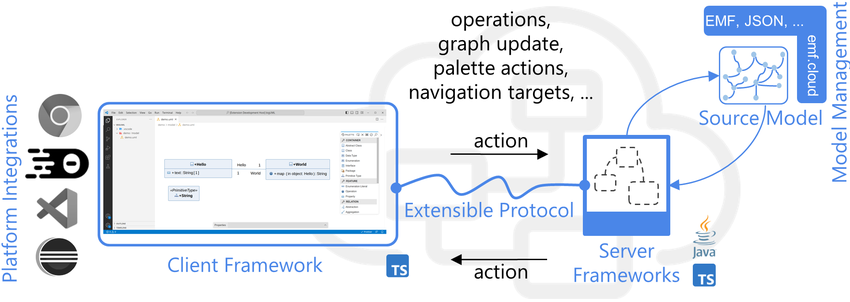
\includegraphics[width=\textwidth]{figures/glsp-overview.png}
	\caption[Overview of GLSP components]{Overview of GLSP components and their interplay. Taken from \cite{bork_vision_2024}.}
    \label{fig:glsp-overview}
\end{figure}

% ----------------------------------------------------------
\subsection{The Graphical Model Transformation Workflow}
\label{subsec:glsp_transformation}
% ----------------------------------------------------------

The architecture of GLSP rests on a two-model abstraction.
The \textit{Source Model} serves as the persistent source of truth and may itself be split into separate domain and notation concerns.
For example, the Eclipse Modeling Framework (EMF) can manage semantic logic independently of visual metadata such as node positions and element dimensions~\cite{metin_developing_2023}.
From the source model, the server derives the \textit{Graphical Model} (GModel), a typed and attributed graph that describes the diagram's structure and geometry.
It serves as the transient artifact exchanged with the client~\cite{bork_vision_2024}.
The natural interaction flow commences by the client encapsulating a user action and sending it to the server for validation and execution rather than applying it as a direct model edit~\cite{bork_vision_2024}.
The server processes the request, potentially modifies the source model, transforms the updated state into a new GModel, and returns it to the client.
The incoming GModel is then rendered as SVG.
This division also reflects a clear authority split: the server determines which elements are rendered based on domain state, while the client controls how they appear through CSS and SVG styling.
For trivial operations such as dragging, the client may apply immediate visual feedback optimistically, with final state reconciliation reserved for the server.
A practical advantage of this architecture is cross-runtime interoperability: a Java-based server can communicate seamlessly with a TypeScript client, allowing complex semantic logic to run on the Java Virtual Machine (JVM) while the user interface remains a responsive web application~\cite{metin_developing_2023, noauthor_eclipse-glspglsp-examples_2026}.

% ==========================================================
\section{Visual Representation Theory}
\label{sec:visual}
% ==========================================================

The choice between textual and graphical representation has measurable consequences for human comprehension and problem-solving efficiency.
Textual representations are inherently one-dimensional and processed serially by the auditory-linguistic system~\cite{larkin_why_1987}.
This requires the reader to hold multiple, potentially distant elements in working memory while searching linearly through the representation.
By contrast, graphical representations are two-dimensional and processed in parallel by the visual system to which approximately a quarter of the brain's total capacity is devoted~\cite{moody_physics_2009}.

The concept of \textit{computational offloading}~\cite{larkin_why_1987} formalises this distinction.
Diagrams index information by spatial location rather than sequential position, allowing elements that must be reasoned about together to be grouped physically.
Spatial, topological, and geometric relationships can thereby be perceived directly, whereas equivalent inferences drawn from text require explicit and effortful computation.
This reduces extraneous cognitive load as identified by Cognitive Load Theory~\cite{sweller_cognitive_2020} and frees working memory for substantive reasoning tasks.

Despite the well-established advantages of graphical representation, the design of visual notations in software engineering has historically been treated as secondary to semantic concerns.
Often it is driven by intuition rather than principled theory~\cite{moody_physics_2009}.
The \textit{Physics of Notations} addresses this deficit by establishing a prescriptive, empirically grounded framework for designing cognitively effective visual languages~\cite{moody_physics_2009}.
The theory derives nine principles from cognitive science and visual perception research~\cite{moody_physics_2009}:
\begin{itemize}
	\item \textbf{Semiotic Clarity:} Each semantic construct should map to one distinct graphical symbol; violations produce redundancy, overload, excess, or deficit.
	\item \textbf{Perceptual Discriminability:} Symbols must be easy to tell apart; discriminability depends on the "visual distance" across variables such as shape, color, and size.
	\item \textbf{Semantic Transparency:} Symbols should visually suggest their meaning so that appearance provides intuitive cues and reduces learning effort.
	\item \textbf{Complexity Management:} Notations should offer mechanisms (for example, modularization, hierarchical grouping, or layered views) to present information incrementally and avoid cognitive overload.
	\item \textbf{Cognitive Integration:} Provide contextual anchors, overview maps, and cross-references so readers can relate individual diagrams to the larger system of representations.
	\item \textbf{Visual Expressiveness:} Leverage multiple visual channels (color, size, brightness, texture, position, etc.) so the notation can encode information across a richer perceptual space.
	\item \textbf{Dual Coding:} Combine concise textual labels or annotations with graphics to leverage both verbal and visual cognitive systems and improve comprehension and retention.
	\item \textbf{Graphic Economy:} Keep the visual vocabulary compact so distinct symbols remain within human discriminative abilities, especially for novice users.
	\item \textbf{Cognitive Fit:} Tailor the notation to task and audience, offering simplified and expert variants so the representation matches users' goals and skills.
\end{itemize}

These principles interact in practice: increasing Visual Expressiveness (e.g., adding color) can improve Perceptual Discriminability and support offset problems introduced by a large graphic vocabulary~\cite{moody_physics_2009}.

% ==========================================================
\section{Drones Example}
\label{sec:bg_drones_example}
% ==========================================================

In the previous sections, we used the mobile phone \gls{uvl} model and the water tank \gls{bp} model as examples.
The drones example, introduced in FMBP~\cite{felber_comprehensible_2025}, serves as a core evaluation use case for the thesis.
It requires interacting with multiple concurrent runtime models, represented by several instances of behavioral programs running simultaneously, which is a key aspect of the thesis.

\lstinputlisting[
    language=UVL, 
    float,
    floatplacement=ht,
    caption={UVL specification of a single drone's feature model. Taken from~\cite{felber_tfelbrfmbp_2025}.}, 
    label={lst:drone_uvl}
]{code/drone.uvl}

The scenario models a small surveillance deployment consisting of four autonomous drones, whose spatial movements and interactions are visualized in real time using an \textit{Alchemist} simulation environment~\cite{pianini_chemical-oriented_2013}.
The swarm's logic is governed entirely by behavioral programming.
Each drone possesses an identical individual feature model represented in \gls{uvl}, which allows capabilities, assignments, and operational parameters to be defined within the model and dynamically applied to each drone at runtime.
Listing~\ref{lst:drone_uvl} shows an example of the \gls{uvl} model for a single drone.
Role assignment is managed through dedicated \textit{Patrol} and \textit{Follow} b-threads, which enforce mutually exclusive behavioral modes.
Drones designated as leaders autonomously navigate and patrol a configurable set of target locations.
In contrast, drones designated as followers are assigned to track a specific other drone, maintaining a configurable separation distance throughout operation~\cite{felber_comprehensible_2025}.

Independently of their assigned role, all drones continuously monitor their internal energy levels through a context-aware energy management mechanism.
When the remaining charge drops below a set threshold, a high-priority 	\textit{Charge} b-thread is activated by a complex constraint.
It overrides the drone's current role and guides it to a designated charging station until its energy is fully replenished.
This mechanism ensures that energy-critical behavior takes precedence over mission-specific tasks across all drone instances at all times~\cite{felber_comprehensible_2025}.

The three used examples, the mobile phone, the water tank, and the drones scenario, are revisited in the evaluation chapter to demonstrate how the proposed toolchain can be applied in practice.